\documentclass[11pt,a4paper]{article}
\usepackage{a4wide}
\usepackage{graphicx}

\begin{document}
\title{\vspace*{-5ex}
Cardiac physiology simulator benchmark for BeatBox}
\author{V. N. Biktashev}
\date{}
\maketitle
\thispagestyle{empty}


Results of the benchmark proposed in ``Verification of cardiac tissue
electrophysiology simulators using an N-version benchmark'' by
S. A. Niederer et al. \textit{Phil. Trans. R. Soc. A} 2011
\textbf{369}, 331-4351, 2011, as performed by BeatBox using
benchmark.bbs in this directory. About the post-processing of the
results, see Makefile.

\bigskip

For figure 2: \\[-1\baselineskip]

\centerline{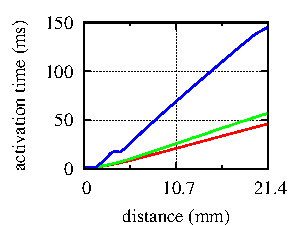
\includegraphics[width=0.4\textwidth]{graph.pdf}}

\bigskip 

For figure 3 (colours selected arbitrary so do not match paper):

\begin{centering}
  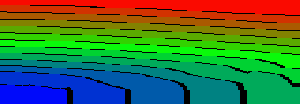
\includegraphics[width=0.4\textwidth]{upper.pdf} \\[1ex]
  
\includegraphics[width=0.4\textwidth]{lower.pdf} \\
\end{centering}

\bigskip 

For the table in the Supplement (note that fig. 4 is only
visualization of the same):

\begin{centering}
\begin{tabular}{l|lllllllll}
  $\Delta x$, $\Delta t$ & $P_1$ & $P_2$ & $P_3$ & $P_4$ & 
  $P_5$ & $P_6$ & $P_7$ & $P_8$ & $C$ \\\hline
  0.1 , 0.005 & 1.22382 & 32.9642 & 9.91335 & 34.3364 & 31.313 & 44.6487 & 32.9291 & 45.6801 & 20.9209 \\\hline
0.1 , 0.01 & 1.22721 & 33.3272 & 9.98596 & 34.7159 & 31.5546 & 45.1389 & 33.2029 & 46.1846 & 21.1429 \\\hline
0.2 , 0.005 & 1.22434 & 35.4602 & 14.0759 & 37.3672 & 42.583 & 55.4801 & 44.7658 & 56.677 & 25.242 \\\hline
0.2 , 0.01 & 1.22771 & 35.7915 & 14.1257 & 37.7231 & 42.7321 & 55.935 & 44.9592 & 57.1537 & 25.4606 \\\hline
0.2 , 0.05 & 1.25431 & 38.3961 & 14.5155 & 40.5161 & 43.9067 & 59.5074 & 46.47 & 60.8908 & 27.1759 \\\hline
0.5 , 0.005 & 1.22551 & 46.8866 & 46.4161 & 64.3489 & 133.489 & 143.851 & 135.663 & 145.399 & 69.1255 \\\hline
0.5 , 0.01 & 1.22887 & 47.0448 & 46.4865 & 64.6528 & 133.63 & 144.184 & 135.831 & 145.752 & 69.3295 \\\hline
0.5 , 0.05 & 1.25543 & 48.2774 & 47.0542 & 67.0577 & 134.755 & 146.829 & 137.152 & 148.555 & 70.9643 \\\hline

\end{tabular}\\
\end{centering}

\bigskip 

The results are similar with other methods using finite differences. 

\end{document}
